\documentclass{article}

\usepackage[latin1]{inputenc}
\usepackage{tikz}
\usetikzlibrary{calc}
\usepackage{tkz-euclide}
\tikzset{line/.style={draw, thick, -latex'}}
%\usetikzlibrary{shapes,arrows}
\begin{document}
\pagestyle{empty}


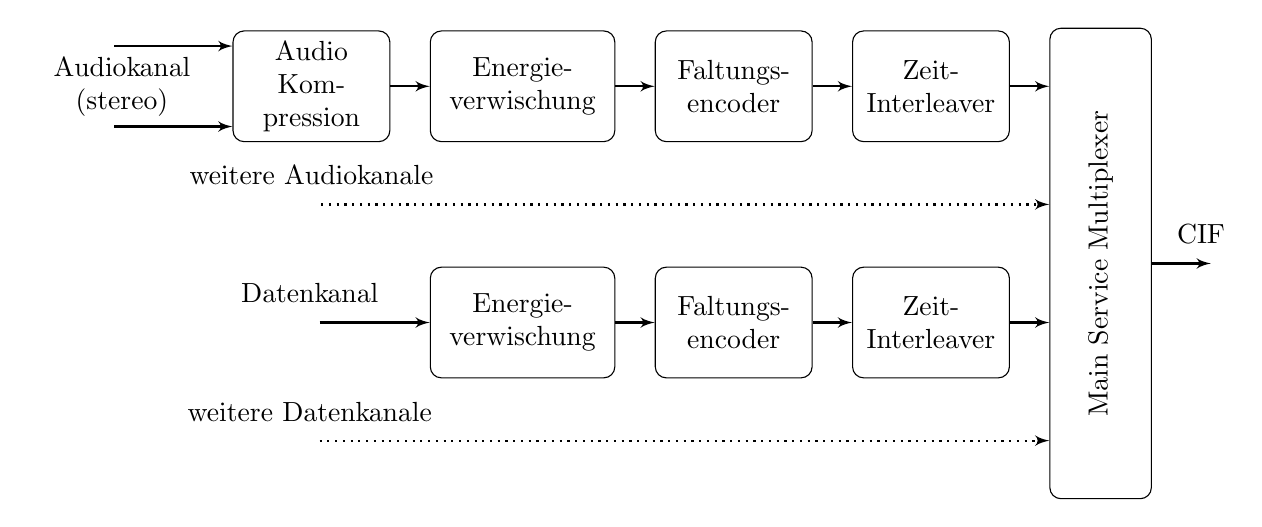
\begin{tikzpicture}
\tikzstyle{block} = [rectangle, rounded corners, draw, text width=5em, text centered, minimum height=4em]
\tikzstyle{input} = [rectangle, text width=0em, minimum height=0em]

% blocks
    % audio1
    \node [](audio1){\begin{tabular}{cc}
Audiokanal \\
(stereo)
\end{tabular}};
    \node [block, right=0.2cm of audio1] (MPEG) {Audio Kompression};
    \node [](audio left)[left=1.5cm of MPEG.153]{};
    \node [](audio right)[left=1.5cm of MPEG.207]{};
    \node [block, right=0.5cm of MPEG, text width=6em] (Energy) {Energie- verwischung};
    \node [block, right=0.5cm of Energy] (conv) {Faltungs- encoder};
    \node [block, right=0.5cm of conv] (time) {Zeit- Interleaver};
    \node [input, right=0.5cm of time](end1){};
    % audioN
    %\node [below=1cm of audio1](audioN){\rotatebox{270}{\dotso}};
    %\node [circle, draw, below of= audio1, node distance = 1.5cm](audioN){};
    \node [below of=MPEG, node distance=1.5cm](audioNpoint){};
    \node [](AudioN text)[above=0cm of audioNpoint]{weitere Audiokanale};
    \node [input, below of=end1, node distance = 1.5cm](end2){};
    % data1
    \node [block, below of = Energy, node distance=3cm, text width=6em] (Energy2) {Energie- verwischung};
    \node [left=1.4cm of Energy2](data1){};
    \node [](Data text)[above=0cm of data1]{Datenkanal};
    \node [block, right=0.5cm of Energy2] (conv2) {Faltungs- encoder};
    \node [block, right=0.5cm of conv2] (time2) {Zeit- Interleaver};
    \node [input, right=0.5cm of time2](end3){};
    % dataN
    \node [below of= data1, node distance = 1.5cm](dataN){};
    \node [](DataN text)[above=0cm of dataN]{weitere Datenkanale};
    \node [input, below of=end3, node distance = 1.5cm](end4){};
    % Mux
    \node [input] (muxpoint) at ($(end1)!0.5!(end4)$){};
    \node [rectangle, rounded corners, draw, text width=3em, text centered, minimum height=17em, left=0.0cm of muxpoint, anchor=west](mux) {\rotatebox{90}{Main Service Multiplexer}};
    \node [](CIF_point)[right=0.5cm of mux]{};
    \node [](CIF)[above=0.0cm of CIF_point]{CIF};
% arrows
    % audio1
    \path [line] (audio left.east) -- (MPEG.west|-audio left);
    \path [line] (audio right.east) -- (MPEG.west|-audio right);
    \path [line] (MPEG.east) -- (Energy.west);
    \path [line] (Energy.east) -- (conv.west);
    \path [line] (conv.east) -- (time.west);
    \path [line] (time.east) -- (end1);
    % audioN
    \path [line, dotted] (audioNpoint.east) -- (end2.west);
    % data1
    \path [line] (data1.east) -- (Energy2.west);
    \path [line] (Energy2.east) -- (conv2.west);
    \path [line] (conv2.east) -- (time2.west);
    \path [line] (time2.east) -- (end3);
    \path [line] (mux.east) -- (CIF_point.east);
    % dataN
    \path [line, dotted] (dataN.east) -- (end4.west);
\end{tikzpicture}
\end{document}